\documentclass{article}
\usepackage{graphicx}
\usepackage{pdfpages}
\usepackage{hyperref}

\hypersetup{
    colorlinks=true,
    linkcolor=blue,
    filecolor=magenta,      
    urlcolor=cyan,
}
\urlstyle{same}
\usepackage[font={small,it}]{caption}
\usepackage{fancyvrb}
\title{Analysis \& Visualization of Call Center Data using Python}
\author{John D. Bulger
\\
Karl Schmitt, PhD. (Advisor)
\\
Valparaiso University\\
}
\date{August 10, 2018}
\begin{document}
\maketitle

\begin{abstract}
\textit{The city of South Bend, Indiana operates a call center that serves as a primary point of contact for citizens.  The call center handles topics for nearly all of the city's departments.  An open data portal, maintained by the city, contains several years worth of information.  An analysis of this data was conducted using Python 3.6.  The data was 
analyzed for patterns by time of year, department, and topics with varying methods.  The cleaned, manipulated, and explored data was then developed into an 
interactive dashboard using the Bokeh library.  In doing so, an interactive HTML file will be distributed to the city, which can then be utilized, modified, and possibly connected 
directly to the data source.  Upon completetion, this analysis yielded} %results stuff here
\end{abstract}

\section{Introduction}
The city of South Bend, located in northern Indiana, established a citizen-accessible call center in February 2013.  The call center handles isues from citizens regarding almost every aspect of city interaction, including waste pick-up and removal, water billing and disconnections, 
and code enforcement.  By serving as a central hub for communication, the call center is able to consolidate a substantial amount of data regarding citizens as consumers.  
This data is available on South Bend's open data portal at \href{https://data-southbend.opendata.arcgis.com}{https://data-southbend.opendata.arcgis.com}.

	\subsection{Prior Work}




	\subsection{Goals \& Desired Results}

The goal of this analysis and visualization task is to, at its core, provide the city of South Bend useful and actionable knowledge about its call center.  Given the information-rich nature of this project, an interactive graphical dashboard was chosen as the primary means to communicate results.  The city was most curious about trends based on time, departments, and topics.  Therefore, this analysis has four major analytical foci:  month of year, day of the week, department, and topic.  


\section{Methods}

	\subsection{Data}

The data to be analyzed was acquired in three distinct comma-separated value files.  Two of the files are publicly available, and are also posted on the \href{https://github.com/jdbul33/verbose-chainsaw}{Github repository} for this project.  The third file was received directly from the city of South Bend, and as a result is not posted publicly at this time.
\par
The first file, referred to as the daily data, contains a daily summary of the call center data from the years 2013-2015.  It is organized with 637 records indexed by date, with each record containing information such as the number of calls presented, average wait time, average number of calls in queue, and number of abandoned calls for that day.
\par
The second file, referred to as the case data, contains 488,601 rows of individual call data from 2013 through 2015.  Calls were logged anonymously with data such as date, duration, topic, and department.  This data format went obsolete when the current call system was implemented.
\par
The third file, referred to as the topic data, is the storage method of the current phone system in use by the city.  This file contains 202,500 call records from 2016-2018.  It contains much of the same attributes as the case data, but it is standardized to reflect the city's use of knowledge base articles.  These articles correspond to possible questions or issues raised by callers; as a result, the call center employees have a reference to answer questions.  Additionally, this systemizes the format for recording issues for each call, since each topic has a standardized name.  This ensures topics and departments match across the list, allowing for efficient and accurate analysis.  Since this is the most recent data and is reflective of the city's current systems, this file was heavily relied upon for analysis on a departmental and topical basis.

	\subsection{Loading, Cleaning, \& Preprocessing the Data}

This entire analysis was completed using the Anaconda 5.2 distribution of Python 3.6.  The data was loaded into 3 separate dataframes through the use of Pandas.  The data was then inspected for missing data and reasonableness.  Very little data was missing, with the exception of a small percentage of observations in the case data (the older data).  Less than 4\% of the 488,601 observations contained missing data.  These rows were missing a significant proportion of their respective attributes, and thus were dropped completely from the data.  The daily data was missing no data points.  The topic data, however, was missing almost 90\% of entries into an attribute titled ``Regarding".  Since this attribute was of type ``string", a substantial amount was missing, and it was irrelevant to the analysis, it was dropped completely.  This dataset was missing no other data.
\par
Upon reading the CSV files using the Pandas, Python initialized most of the attributes as objects.  Preprocessing and transforming was conducted immediately to transform the attributes into more useful types, such as date-time and numeric objects.  Further processing was done throughout the project as necessary in order to provide a useful format.

	\subsection{Methods of Analysis}

An analysis of call volume by month was conducted using the daily data, which provides aggregate totals by day for a 2-year period. The relevant data was manipulated by taking the mean of the daily call volume for every record in each month.  As an exercise in thoroughness, these findings were subjected to a two-sided t-test for statistical significance.  The daily call volumes for each month were isolated and stored as lists within a Python dictionary.  The scipy.stats package was used to conduct the test.  For the purposes of this test, the null hypothesis stated that ``the two months have identical expected values."  For the null hypothesis to be disproved, a standard threshold p-value of 0.05 was used.

	\subsection{Calls by Day of Week}

Calls by day of week were able to be obtained from two data files:  daily data and topic data.  The first conveniently had an attribute consisting of an integer corresponding to a weekday.  The topic data included a date of call, but it did not have a direct day attribute.  Such an attribute was able to be created through the use of the ``to\_datetime()" and ``weekday()" functions in Pandas.  Once this attribute was created in the same format as the daily data, the dataframes were concatonated using ``concat()".  Aggregate call totals by day were then simply calculated using the ``.count()" method in Pandas.

	\subsection{Calls by Department}

One of the primary tasks posed by the city was to explore call trends on a departmental level.  This was conducted primarily using the topic data, as the data contained accurate and complete information regarding departments.  In addition to being the most recent, this data also utilizes the new department/topic layout that the city has transitioned to.  This format includes the knowledge base articles described earlier.  In this native data format, the department titles were often followed by the characters ``- KB Team".  Since leaving this suffix appended to each title would only visually detract from the dashboard, the string was removed.  
\par
Additionally, the time format in the data file was read in as a string.  Upon investigating, the data was found to have an inconsistent format.  For example, duration for one record was in the form ``2:34" for two minutes, thirty-four seconds.  However, for longer calls it could be in the form ``1:15:56" for one hour, fifteen minutes, and fifty-six seconds.  While beneficial visually, this would not function for any analysis.  This data was converted into seconds, and stored as a numeric data type.

	\subsection{Calls by Topic}

The topic data was used again here due to its recentness and the homogeneity of topic format.  Among this dataset, 426 unique call topics existed.  The data was then processed to show total call count and average call duration by topics.  This data was then merged with a separate dataframe, indexed by topic with department as the only attribute.  Once completed, the resulting dataframe contained topic, count, average call duration, and corresponding department.  At this point, the data was prepared for analysis.
\par
Call duration by topics was calculated in the dataframe creation above, using the ``.groupby()'' method in Pandas.  However, when the dataframe was sorted to see the quickest and longest average duration, several topics with a low volume rose to the top, some with only one total call.  In a sense, such records can be viewed as outliers, and were thus removed from reporting in the final dashboard.  In the end, only topics with a total volume above the first quartile (of total calls) were included in this analysis.  By reducing the topics analyzed, the call center will be able to focus on topics that take a notable duration to resolve, but that also occur frequently enough to warrant attention.  This code, however, can be easily adjusted to a different threshold, if management so desires.
\par
The total number of calls by topic was then analyzed.  The dataframe that was used in the previous analysis was again used for this.  Using the ``.groupby()" method in Pandas in conjunction with ``.count()", the total number of calls for each topic was appended to the dataframe.  The most frequent call topics were quickly identified, and many showed a significant overlap with the highest volume departments.  As a result, the volume by topic in and of itself would not serve much use to the city.  Therefore, the top 7 highest volume departments (identified in Figure 2) were isolated from the rest of the data.  The individual topics within these departments were then identified.  By approaching the analysis in this manner, the city can easily see the most popular topics in the busiest departments.



\section{Analysis}

	\subsection{Calls by Month}

Upon analysis, the months with the highest average daily call volumes were July, April, Jun, and May (in that order).  The results can be viewed in Figure 1.  The standard errors for each month (also plotted in Figure 1) do not appear to be so large as to discredit the significance of these differences.  March, interestingly, has the lowest average volume by a large margin.  This is especially intriguing since it is immediately prior to what can be seen as the ``busy season".

The heatmap in Figure 2 shows the resulting p-value between each pairing of months.  From this information, the city can see which months are significantly busier/quieter than others.  By subjecting the data to such a test, important points can be quickly identified that may or may not be obvious in Figure 1.  For example, June's call volumes are not statistically different from those in April.  March, however, has a statistically lower daily average than every other month.


	\subsection{Calls by Day}

The analysis of calls by day of week incorporated over 588,000 calls into the results.  The output, therefore, can be viewed as information-rich and an excellent measure of call center activity, since the combined data sources span from 2013 into 2018.  Given the variablity of the vast amount of data, an interactive historgram was chosen as the best method for communication of results.  The user can click to show/hide days of the week, and the chart will layer the call distributions over each other for comparison.  Figure 3 shows this graph, with Monday and Thursday visible.  The general call distribution of each day is similar and appears to follow a 
%what the hell kind
distribution.  Monday has the highest volume distribution, while Friday has the lowest.  This is also evidenced in a swarm plot of only the daily data in Figure 4.


	\subsection{Calls by Department}

Calls by department were analyzed by two measures:  average duration and total volume.  As expected, the results of each analysis differed.  Departments such as Solid Waste and Water Works had the highest call volumes, while Code Enforcement and the Mayor's Office has the longest average durations.  Given this incongruency, it is not immediately clear where the call center's resources are being focused.  As a more direct approach to the measure of total call volume, the total departmental call times were calculated.  Of all the approaches, this calculation of total call time may be the most helpful to the city, as this can directly show where time and budget is being spent.


	\subsection{Calls by Topic}

Exploration of calls by topic was a priority for the city.  Within each department, numerous topics exist.  Given the recent implementation of knowledge base articles (which can be seen in the most recent data), the attachment of topics to each call has been standardized.  This allows for a simplified, more accurate analysis.  Calls by topic were specifically analyzed by average duration and total call volume.
\par
The %left off here

\section{Discussion}

	\subsection{Final Dashboard}

After completion of the above analysis, the final dashboard was constructed.  Each chart in this dashboard stems from a question or interest identified by the city analysts.  The Bokeh package was used to create interactive visualizations, and allowed the final product to be conveniently packaged into a HTML file and sent to the call center management.  In all, the dashboard includes visualizations of:

\begin{itemize}
  \item{Pie chart of total call time by department}
  \item{Histogram of call volume by day of week, overlaid, with legend providing hide/show capabilities}
  \item{Bar chart of topics with longest average call duration}
  \item{Bar chart of topics with shortest average call duration}
  \item{Jitterplot of call volume by topic within top departments}
  \item{Bar chart of call volume by month}
\end{itemize}

These charts all utilize various implementation of Bokeh tools, such as HoverTool, BoxZoom, Pan, and checkbox interactivity.  By incorporating these interactions into the dashboard, the result is a more dynamic, engaging product that is simple to interact with for employees outside of the technical fields.  An image of the final dashboard can be found at the end of this paper, while a live link can be followed \href{https://jdbul33.github.io/311_Call_Dashboard.html}{here}.


\section{Conclusions}

In summary, this analysis and presentation of data trends can be viewed as a successful high-level exploration.  Trends and points emerged from this analysis that will surely be of interest to call center management, while more insights can surely be found while interacting with the visualization dashboard.  For the city, this study should serve to identify areas of business interest within the context of these findings, which could then warrant further exploration with more specific questions.  For example, the city may want to see day-of-week trends for a specific topic, or they may seek to see how the number of calls queued relate to the number of calls abandoned.  These more specific questions would necessarily arise from a specific business need, which could perhaps be identified from this study.

	\subsection{Opportunities for Further Work}

Several paths for further work on this topic exist; however, the exact approach depends on the city's desires.  One approach would be to obtain staffing and scheduling information for the call center and use simulation and optimization techniques to evaluate staffing levels and efficiency.  Another approach would be to develop another dashboard, or perhaps modify the current one, to interact directly with the call center's data source.  This would allow a live, current view of trending topics and departments.  Such a tool could allow call center management to be agile and preemptive regarding emerging trends.



\begin{thebibliography}{9}
	
\bibitem{python}
Python Software Foundation. (2016). Python 3.6. https://docs.python.org/3.6/.

\bibitem{anaconda}
Anaconda. (2018). Anaconda Distribution 5.2. https://docs.anaconda.com/anaconda/.


\end{thebibliography}
\newpage

\begin{figure}[p]
  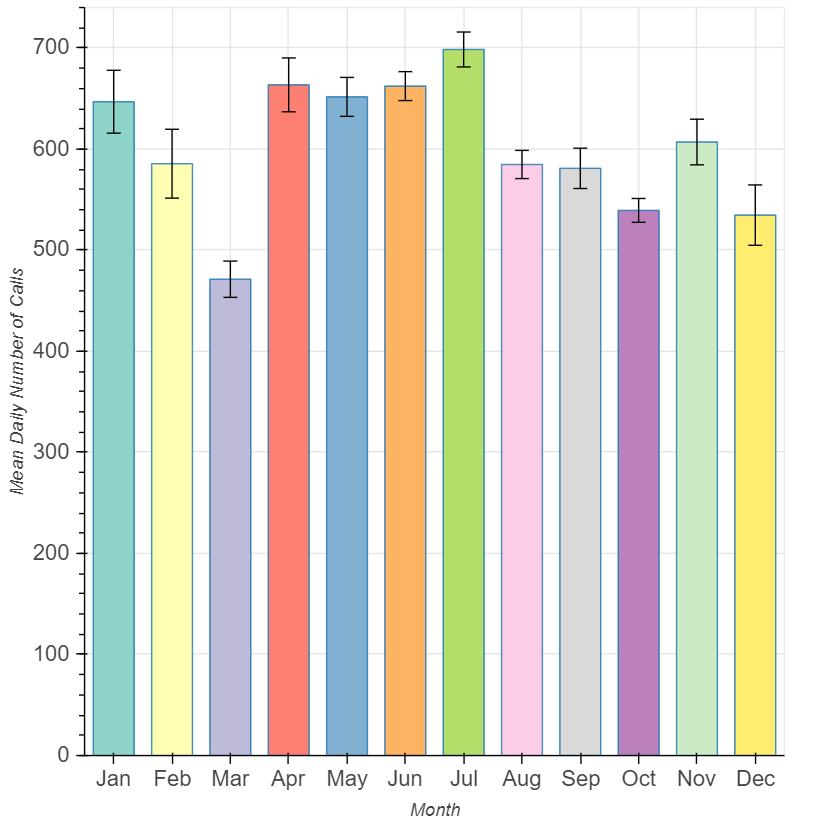
\includegraphics[scale=.27]{month_bar.png}
  \caption{Plot of average daily call volume by month}
\end{figure}

\begin{figure}[p]
	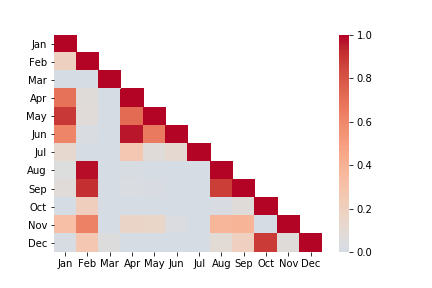
\includegraphics[scale=.5]{Heatmap.png}
	\caption{P-values resulting from t-test on daily call volume by month}
\end{figure}


\begin{figure}[p]
	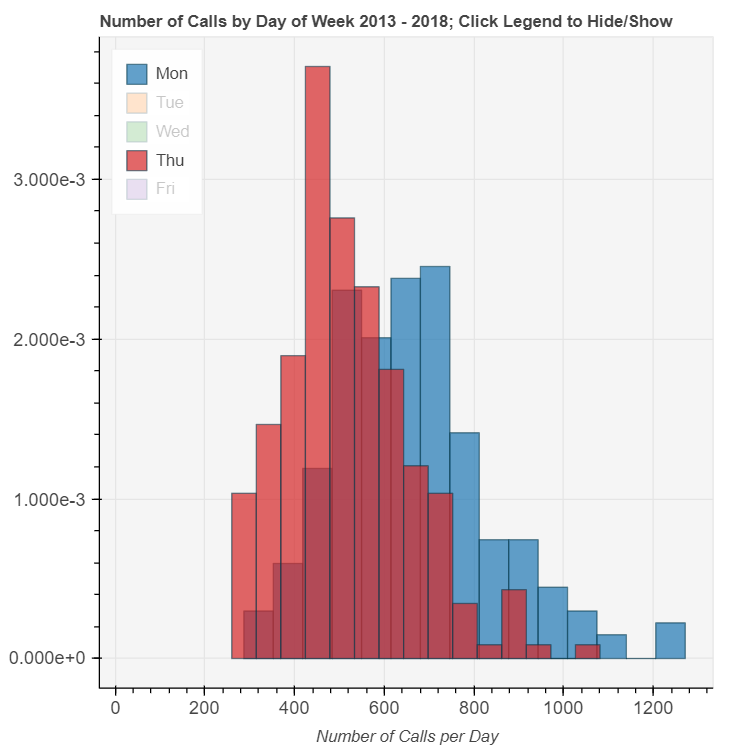
\includegraphics[scale=.35]{daily_calls.png}
	\caption{Histogram of total daily calls by day of week, 2013-2018}
\end{figure}

\begin{figure}[p]
	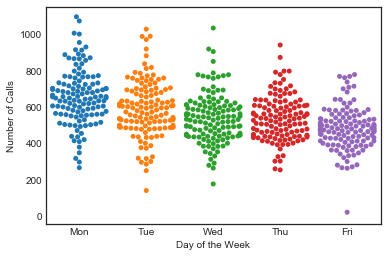
\includegraphics[scale=.6]{swarm.png}
	\caption{Swarmplot of total daily calls by day of week, 2013-2015}
\end{figure}

\begin{figure}[p]
  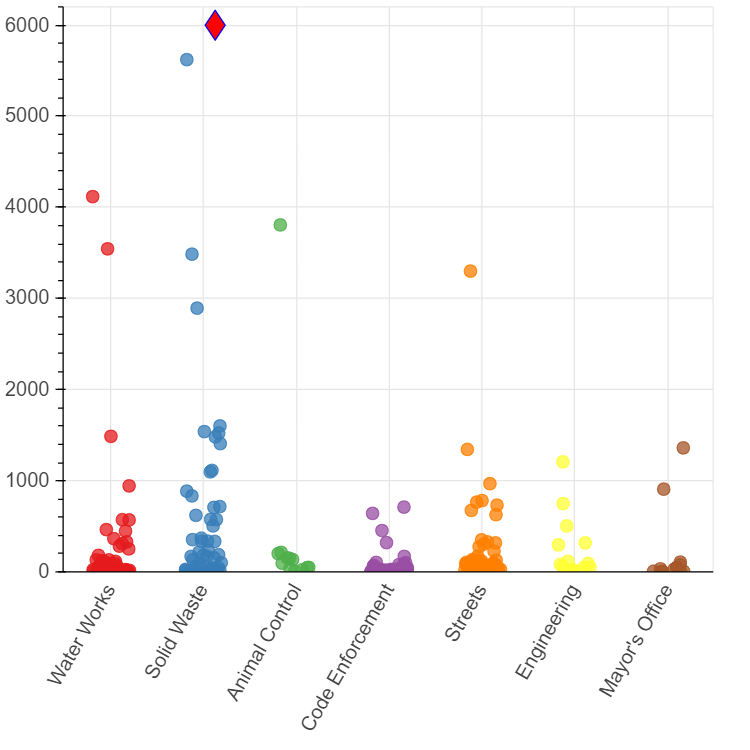
\includegraphics[scale=0.25]{jitterplot.png}
  \caption{Jitterplot of call volume by topic for the busiest departments.  Hovertool is utilized to show topic.  The topic in diamond is not plotted to scale}
\end{figure}

\end{document}

